\documentclass[a4paper]{artikel1}
\usepackage{lmodern}
\usepackage{amssymb,amsmath}
\usepackage{ifxetex,ifluatex}
\usepackage{fixltx2e} % provides \textsubscript
\ifnum 0\ifxetex 1\fi\ifluatex 1\fi=0 % if pdftex
  \usepackage[T1]{fontenc}
  \usepackage[utf8]{inputenc}
\else % if luatex or xelatex
  \ifxetex
    \usepackage{mathspec}
  \else
    \usepackage{fontspec}
  \fi
  \defaultfontfeatures{Ligatures=TeX,Scale=MatchLowercase}
\fi
% use upquote if available, for straight quotes in verbatim environments
\IfFileExists{upquote.sty}{\usepackage{upquote}}{}
% use microtype if available
\IfFileExists{microtype.sty}{%
\usepackage{microtype}
\UseMicrotypeSet[protrusion]{basicmath} % disable protrusion for tt fonts
}{}
\usepackage[margin=1in]{geometry}
\usepackage{hyperref}
\hypersetup{unicode=true,
            pdftitle={Keystoneness, centrality, and the structural controllability of ecological networks},
            pdfauthor={Fernando Cagua, Kate L. Wootton, Daniel B. Stouffer},
            pdfborder={0 0 0},
            breaklinks=true}
\urlstyle{same}  % don't use monospace font for urls
\usepackage{longtable,booktabs}
\usepackage{graphicx,grffile}
\makeatletter
\def\maxwidth{\ifdim\Gin@nat@width>\linewidth\linewidth\else\Gin@nat@width\fi}
\def\maxheight{\ifdim\Gin@nat@height>\textheight\textheight\else\Gin@nat@height\fi}
\makeatother
% Scale images if necessary, so that they will not overflow the page
% margins by default, and it is still possible to overwrite the defaults
% using explicit options in \includegraphics[width, height, ...]{}
\setkeys{Gin}{width=\maxwidth,height=\maxheight,keepaspectratio}
\IfFileExists{parskip.sty}{%
\usepackage{parskip}
}{% else
\setlength{\parindent}{0pt}
\setlength{\parskip}{6pt plus 2pt minus 1pt}
}
\setlength{\emergencystretch}{3em}  % prevent overfull lines
\providecommand{\tightlist}{%
  \setlength{\itemsep}{0pt}\setlength{\parskip}{0pt}}
\setcounter{secnumdepth}{0}
% Redefines (sub)paragraphs to behave more like sections
\ifx\paragraph\undefined\else
\let\oldparagraph\paragraph
\renewcommand{\paragraph}[1]{\oldparagraph{#1}\mbox{}}
\fi
\ifx\subparagraph\undefined\else
\let\oldsubparagraph\subparagraph
\renewcommand{\subparagraph}[1]{\oldsubparagraph{#1}\mbox{}}
\fi

%%% Use protect on footnotes to avoid problems with footnotes in titles
\let\rmarkdownfootnote\footnote%
\def\footnote{\protect\rmarkdownfootnote}

%%% Change title format to be more compact
\usepackage{titling}

% Create subtitle command for use in maketitle
\newcommand{\subtitle}[1]{
  \posttitle{
    \begin{center}\large#1\end{center}
    }
}

\setlength{\droptitle}{-2em}
  \title{Keystoneness, centrality, and the structural controllability of
ecological networks}
  \pretitle{\vspace{\droptitle}\centering\huge}
  \posttitle{\par}
\subtitle{JEcol-2018-0545 - Detailed response to comments}
  \author{Fernando Cagua, Kate L. Wootton, Daniel B. Stouffer}
  \preauthor{\centering\large\emph}
  \postauthor{\par}
  \date{}
  \predate{}\postdate{}

\usepackage{setspace}
\usepackage{xr}
\usepackage{lineno}
\newcommand{\R}[1]{\label{#1}\linelabel{#1}}
\newcommand{\lr}[1]{page~\pageref{#1}, line~\lineref{#1}}
\externaldocument[M-]{manuscript}
\externaldocument[S-]{supp-info}
\usepackage[most]{tcolorbox}
\definecolor{block-gray}{gray}{0.9}
\newtcolorbox{myquote}{colback=block-gray,grow to right by=-10mm,grow to left by=-10mm, boxrule=0pt,boxsep=0pt,breakable}

\usepackage{amsthm}
\newtheorem{theorem}{Theorem}
\newtheorem{lemma}{Lemma}
\theoremstyle{definition}
\newtheorem{definition}{Definition}
\newtheorem{corollary}{Corollary}
\newtheorem{proposition}{Proposition}
\theoremstyle{definition}
\newtheorem{example}{Example}
\theoremstyle{definition}
\newtheorem{exercise}{Exercise}
\theoremstyle{remark}
\newtheorem*{remark}{Remark}
\newtheorem*{solution}{Solution}
\begin{document}
\maketitle

\renewcommand\thefigure{R\arabic{figure}}    

\setcounter{figure}{0}

\doublespacing

We are thankful to the assistant editor James Ross, the senior editor
and David Gibson, and three anonymous reviewers for the insightful
comments to improve the manuscript. In the following sections, you can
find a detailed response to each comment raised during the previous
round of review.

\section{Editor comments}\label{editor-comments}

\begin{quote}
``I agree that your manuscript is much improved and now only in need of
relatively minor revisions. In addition to addressing the AE and
reviewer's comments, please add terms related to invasive species to the
keywords to aid in discoverability of your paper.''
\end{quote}

Many thanks for the encouraging words. We have included `invasive
species' as a keyword. To make space for this keyword we have removed
`controllability' which is already highlighted as part of the title.

\section{Associate Editor's comments}\label{associate-editors-comments}

\begin{quote}
``I think this ms now makes much clearer the potential insights to be
gained by applying control theory to interaction networks. In
particular, the authors have done a nice job of explaining how their
findings reinforce existing ideas in the literature on the stability of
ecological networks while also acknowledging limitations. The reviewers
identified a few remaining issues that should be straightforward to
address. I also noticed a few issues''
\end{quote}

Thank you for the positive feedback. We have addressed all of the
specific issues raised and highlight these in red text in our
resubmitted manuscript.

\begin{quote}
``\emph{L9}: I think here and throughout much of the text, species
should be possessive when followed by a noun (''species role" should be
``species' role''). The possessive is currently used in some instances
but is inconsistently applied throughout the ms."
\end{quote}

\emph{Accepted and changed}. We have checked through the manuscript and
corrected this where relevant. Besides \emph{specie's role}, we also
changed instances of \emph{species' contribution}, \emph{species'
degree}, \emph{species' control capacity}, among others.

\begin{quote}
``\emph{L25}: `every invasive species in our dataset was part of it'
Here it was unclear what `it' refers to (the set of critical species),
and the reference to a singular dataset when you have 20 networks in
total was a bit confusing to me.''
\end{quote}

\emph{Accepted and changed}. We have made this clearer as follows: ``and
included every invasive species in our dataset''
(\lr{M-R2-our-dataset}).

\begin{quote}
``\emph{L23-26}: in these lines, you refer to critical species, but I
think the distinction between having high control capacity versus being
critical needs to be defined (briefly) earlier (it is stated in
\emph{L18-19} that you will quantify both control capacity and identify
critical species, but it is not explained how they are distinct).''
\end{quote}

\emph{Accepted and changed}. We now identify the distinction between
high control capacity and being critical on
\lr{M-R2-define-control-capacity}. The text now reads ``It also allows
us to quantify a species control capacity-its relative importance-and
identify the set of species that, collectively, are critical in this
context because they have largest possible control capacity''.

\begin{quote}
``\emph{L27}: unclear what `its' refers to.''
\end{quote}

\emph{Accepted and changed}. We now explicitly state ``species' degree''
in \lr{M-R2-species-degree}.

\begin{quote}
``\emph{L234, 235}: awkward to refer to species as `they' and
`their'\,''
\end{quote}

\emph{Accepted and changed}. We have changed this to ``it'' and ``its''.

\begin{quote}
``\emph{L296}: `More details in Supporting Information.' is a sentence
fragment.''
\end{quote}

\emph{Accepted and changed}. We have corrected this on
\lr{M-R2-sentence-fragment}. The text now reads ``See Supporting
Information Section \ref{S-visitation-as-proxy} for more details''.

\begin{quote}
``\emph{L343}: I am not sure about citing Table 2 for the first time in
the Discussion. Might it be more useful to cite this in the
Introduction?''
\end{quote}

\emph{Accepted and changed}. We now introduce the glossary at the end of
the introduction on \lr{M-R2-ref-glossary}.

\begin{quote}
``\emph{L111, 114}: `are comprised of' should be `comprised'.
\emph{L339, 432}: `at' should be `in'. \emph{L341}: `allow' should be
`allowed'. \emph{L355}: missing period.''
\end{quote}

\emph{Accepted and changed}. Thank you for pointing out these mistakes,
we corrected all of them.

\section{Reviewer comments \#1}\label{reviewer-comments-1}

\begin{quote}
``I'd like to commend the authors to this revised version of the
manuscript on `Keystoneness, centrality, and the structural
controllability of ecological networks'. I thoroughly enjoyed the
re-written manuscript, which is now considerably more accessible and
clearly targets the community of network ecologists, while not ignoring
the importance of the applied relevance of the findings. Overall, I
don't have any major comments. I guess the language is in parts on the
casual side, yet without compromising the preciseness or clarity of the
text. I noticed a few typos or style errors that the authors may want to
address. Congratulations on this thought-provoking methodological
synthesis.''
\end{quote}

We are pleased that the reviewer enjoyed the re-written manuscript. We
did too!. We also grateful for the typos and style errors identified, we
have striven to correct them all.

\begin{quote}
``A few references require editing to journal style (e.g.~remove
initials for many citations)''
\end{quote}

\emph{Accepted and changed}. We have corrected all citations. One of
them, however, still shows an author's first name initial, as it is
necessary to distinguish two authors with the same last name
(\lr{M-R2-citation-with-name}).

\begin{quote}
``\emph{L388}: remove repeated `other'. I suggest that the authors
re-write this sentence to improve clarity.''
\end{quote}

\emph{Accepted and changed}. We have removed the second `other'. As
suggested, we have rewritten the sentence to improve clarity
(\lr{M-R2-structural-controllability}). It now reads as follows:
``First, structural controllability emphasizes that the effect a species
has on the abundance of other species is not independent of the effects
of those other species in their community''.

\begin{quote}
``Reference list needs updating, e.g.~Ne'eman et al. is not 2009 but
2010.''
\end{quote}

\emph{Accepted and changed}. Thanks for pointing this error out. We've
corrected the reference.

\begin{quote}
``\emph{L314}: open bracket missing. \emph{L358}: change `instead' to
`Instead'. \emph{L381}: remove second comma. \emph{Fig. S6} header of
plot b). correct spelling of `critical'.''
\end{quote}

\emph{Accepted and changed}. Thank you for pointing this out, made all
these changes as indicated.

\section{Reviewer comments \#2}\label{reviewer-comments-2}

\begin{quote}
``I think the concepts presented in this manuscript are a useful
addition to the literature on management of ecological networks. I agree
with the authors that it is important that the discussion surrounding
what constitutes a `keystone' species should go beyond centrality
metrics. I found the results and concepts to be generally well
presented, particularly graphically, and the authors present a thorough
sensitivity analysis to various assumptions.
\end{quote}

We are very thankful for the positive feedback but also for the issues
highlighted. We have aimed to address them all.

\begin{quote}
``The methods are mostly clear but there is no description of how the
`likelihood of being a superior node' is calculated.''
\end{quote}

\emph{Accepted and changed}. Thanks for pointing this out. We have
modified the sentence mentioning `the likelihood of being a superior
node' in the first paragraph of the section \ref{S-reciprocal-links} to
``\ldots{}and whether it is a superior node\ldots{}'' to avoid
confusion. Then we define the `probability of being a superior node' at
the end of the section: ``It is important to note that a species that is
found to be a superior node under a particular control configuration,
will be so in all possible control configurations for the particular
non-reciprocal network. We, therefore denote the average of \(\sigma\)
across all non-reciprocal versions as the probability of the species
being a superior node in its community''.

\begin{quote}
``I would suggest including clarification on the limitations of using
control capacity to summarise species' importance, and examples to help
the reader build an intuition regarding the control capacity metric. As
pointed out, networks that give rise to a species having a high control
capacity can be quite distinct to networks that give rise to a species
having a high value of particular centrality metrics. Providing an
example in the Discussion of, for instance, those species that have a
control capacity of 1 but a low degree would be very useful.''
\end{quote}

\emph{Need Daniel's input}

\begin{quote}
``Jargon occasionally obfuscates the concepts being introduced and there
are places where I thought the language used was vague (esp. if terms
being used have particular meanings depending on the field you're coming
from). I would suggest clarifying, or rewording, the following: `desired
control trajectory' - does this mean `final state'?''"
\end{quote}

\emph{Accepted and changed}: We have attempted to clarify this sentence
as follows: Finding out exactly how difficult it is to control a network
depends strongly on the particularities of the desired control
trajectory (i.e.~the path to the desired final state) as well as the
dynamical relationship between nodes.
\lr{M-R2-desired-control-trajectory}.

\begin{quote}
``\emph{L1364}: `dynamic persistence'\,''
\end{quote}

\emph{Accepted and changed}: Thank you. To avoid confusion we have
removed the word `dynamic' and now the sentence reads ``\ldots{}our
results suggest that structural controllability is closely related to
the persistence\ldots{}'' (\lr{M-R2-dynamic-persistence}). It conserves
its meaning without losing much precision.

\begin{quote}
``\emph{L1370}: `dynamic stability'\,''
\end{quote}

\emph{Accepted and changed}: Contrastingly, in this case the word
dynamic distinguishes a particular facet of stability. We mean the
ability of the system to return to an equilibrium state after a
perturbation. We now include this definition on
\lr{M-R2-dynamic-stability} to make the concept clearer.

\begin{quote}
``\emph{P9}: `ecological objective' - simply `objective'?''
\end{quote}

\emph{Accepted and changed}: We have changed this to simply `objective',
as suggested (\lr{M-R2-ecol-objective}).

\begin{quote}
``\emph{L405}: `central in their community'\,''
\end{quote}

\emph{Accepted and changed}: We've changed the wording to avoid
ambiguity. Now the text reads ``\ldots{}to attain high centrality in
their communities\ldots{}'' (\lr{M-R2-central-in-their-communities}).

\begin{quote}
``\emph{L406}: 'inherently different. The sentence spanning lines
407-410 is quite confusing - please clarify.
\end{quote}

\emph{Accepted and changed}: We rephrased this line as follows: ``We
found that it is not that invasive plants have some different mechanism
for influencing the community compared to their native counterparts''
\lr{M-R2-inherrently-different}.

\begin{quote}
``\emph{L430}: `marginally affected by the topology of their
interactions'\,''
\end{quote}

\emph{Accepted and changed}: We have rephrased this line as: ``By
accounting for network dynamics (even if in a simple way), structural
stability incorporates more ecological realism, especially in the
extreme scenario in which the structure of interactions within the
community only marginally affects the community's state. Both native
species and invasive plants tended to attain a high control capacity if
they were important to network persistence, were abundant, and depended
little on other species'' (\lr{M-R2-marginally-affected}).

\begin{quote}
``\emph{L436} and \emph{L441}: `dominate the state {[}of their
community{]}'\,''
\end{quote}

\emph{Need Daniel's input}

\begin{quote}
``\emph{Discussion}: `species' strength'''
\end{quote}

\emph{Accepted and changed}: In the Methods section we deine species'
strength as the sum of a species' visits (\lr{M-R2-species-strength-a}).
For brevity, we did not define it again in the Discussion, but now we
have improved the text and briefly describe it when we mention it there
too. The text now reads ``When controlling for a species' visitation
strength (the sum of a species' visits), which is indirectly a proxy of
its abundance\ldots{}'' (\lr{M-R2-species-strength-b}).

\begin{quote}
``Minor typos: \emph{Figure S11} caption: `likelyhood' -\textgreater{}
likelihood. \emph{L388}: `other other'. `Driver node density' (supp p12)
-\textgreater{} `size of the minimum driver node set'?''
\end{quote}

\emph{Accepted and changed}: All typos have been corrected as indicated.

\begin{quote}
``\emph{Figure S1b} is referred to (supp. p4 ) but doesn't exist in the
figure''
\end{quote}

\emph{Accepted and changed}: Thanks for noticing this issue. We now
refer to the figure as ``Figure S1 (center panel)''.

\begin{quote}
``\emph{References}: several references use the term `plantPollinator',
or `\ldots{}'\,''
\end{quote}

\emph{Accepted and changed}: We have corrected the reference that
included `plantPollinator' in the title. We have left the references
that include an ellipsis in the author list as they are, as the Journal
of Ecology Author Guidelines indicate that this is the preferred format
when the reference has more than seven authors.

\section{Reviewer comments \#3}\label{reviewer-comments-3}

\begin{quote}
``In the literature on ecological networks, the term keystone species
has often been tossed around without any clear definition. I was pleased
to read that here the authors have developed a cleaner, more effective
way to identify keystone species in ecological networks than methods
that have been proposed before. I think the authors have made the
correct choice in emphasizing the conceptual aspects of the approach,
and do so quite well. The background on control theory was complex but
manageable to read and understand in this context.''
\end{quote}

We are very thankful for the positive feedback.

\begin{quote}
``Overall I found the paper well-written and sound, but there were a few
questions I had that could improve clarity in the methods used. In the
glm that used nD as the response variable, is there any concern that
including N (number of species) as a predictor may cause a problem when
the response is D/N? I can understand why this was included, but I can
also imagine this resulting in models that show an effect of N when
there is none (I could be wrong on this).''
\end{quote}

\emph{Need Daniel's input}

\begin{quote}
``In the species level glm, it was not entirely clear if models were fit
to each network individually or if all species were lumped together (the
former is what I think was done based on my reading of the text).
Regardless I wonder if it would change the results if a mixed effects
model was fit to lumped data, using network as a random effect.''
\end{quote}

\emph{Accepted and changed}: We are sorry for the confusion. In the
species level GLM, we lumped all species from different networks
together. We have modified the text in \lr{M-R2-one-lumped-model-a} and
\lr{M-R2-one-lumped-model-b} to make this clearer. We actually did test
for random effects in the model. We tested random effects that allowed
for a random intercept for the network (but also its site, and the study
it comes from). In all cases, the variance among groups was zero. This
means that likely there are no differences on the distribution of
control capacity between networks (or site and study) and therefore it
was not necessary to include random effects in the models presented in
the paper. We have corrected this omission and describe the random
effects in \lr{M-R2-random-effects}.

\begin{quote}
``How were the model sets derived? Were all possible sub-models compared
or was a step-wise approach used?''
\end{quote}

\emph{Accepted and changed}: We actually compared all possible candidate
models. We have edited the manuscript on \lr{M-R2-all-candidates} to
include this information.

\begin{quote}
``Reciprocal links were included in the directed graph when dij = dji.
Would it have any effect if there was a little wiggle room there, e.g.,
when the two are close but not equal?''
\end{quote}

We did not actually evaluate this When we evaluate the impact of this on
our results. However, given that the interaction only a very small
fraction of interactions had a small asymmetry (see Figure R1) we don't
expect results to change considerably even when we include reciprocal
links when the asymmetry is small but not zero.

\begin{figure}
\centering
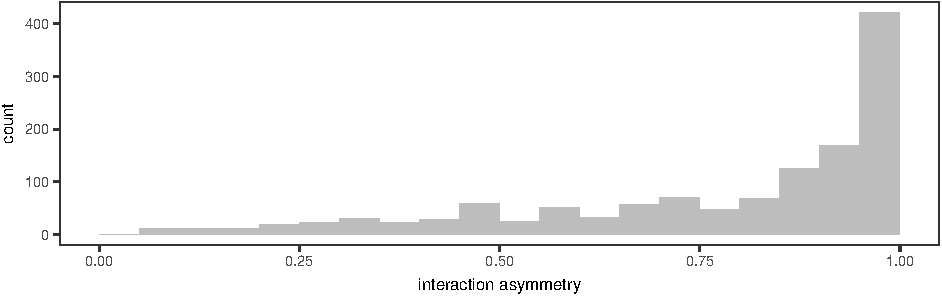
\includegraphics{/Users/efc29/github/driver-species/paper/reviewers-response_files/figure-latex/fig-asymmetry-1.pdf}
\caption{\label{fig:fig-asymmetry}Histogram of the interaction asymmetries
between species. Previous research has shown that mutualistic
interactions are often highly asymmetric in natural communities. Only
16.5\% of interactions have asymetries smaller or equal than 0.5; 1\%
are smaller than 0.1.}
\end{figure}


\end{document}
